\documentclass{article}


\usepackage{arxiv}

\usepackage[utf8]{inputenc} % allow utf-8 input
\usepackage[T1]{fontenc}    % use 8-bit T1 fonts
\usepackage{hyperref}       % hyperlinks
\usepackage{url}            % simple URL typesetting
\usepackage{geometry}
\geometry{margin=0.5in}
\usepackage{multirow}
\usepackage{float}
\usepackage{graphicx}
\usepackage{caption}
\usepackage{filecontents}
\usepackage{subcaption} % Add the subcaption package
\usepackage[title]{appendix}
\usepackage{fancyhdr}
\usepackage{array}
\usepackage{booktabs}       % professional-quality tables
\usepackage{amsfonts}       % blackboard math symbols
\usepackage{nicefrac}       % compact symbols for 1/2, etc.
\usepackage{microtype}      % microtypography
\usepackage{lipsum}
\usepackage{graphicx}
\pagestyle{fancy}
\usepackage{amsmath}
\graphicspath{ {./images/} }
\usepackage[compact]{titlesec}         % you need this package
\titlespacing{\subsection}{0pt}{5pt}{0pt} % this reduces space between (sub)sections to 0pt, for example


\title{COMP 551 Assignment 2 Report - Fall 2024}


\author{
 Hathaway Hao \\
  261071268\\
  %% examples of more authors
   \And
 Yifan Lin \\
  261078741\\
  \And
 Michael Yu \\
  261070826\\
  %% \AND
  %% Coauthor \\
  %% Affiliation \\
  %% Address \\
  %% \texttt{email} \\
  %% \And
  %% Coauthor \\
  %% Affiliation \\
  %% Address \\
  %% \texttt{email} \\
  %% \And
  %% Coauthor \\
  %% Affiliation \\
  %% Address \\
  %% \texttt{email} \\
}

\begin{document}
\maketitle
\begin{abstract}
\textit {Statistical learning is key to Machine Learning}

\end{abstract}



\section{Task 1: Linear Regression with Non-Linear Basis Functions}

\subsection{Introduction}
\noindent The main objective of Task 1 is to explore the effectiveness of Gaussian basis functions in approximating non-linear relationships. We aim to demonstrate how increasing the complexity of a model by adding more basis functions affects its performance, highlighting the trade-off between underfitting and overfitting. Our approach starts with generating synthetic data from a non-linear function, and then attempting to approximate this function using a linear combination of Gaussian basis functions. We then can observe how model complexity by changing the number of basis functions, which influences the quality of fit and generalization performances.


\subsection{Methodology}
\paragraph{Data Generation}
We begin by generating a synthetic dataset that represents a non-linear relationship. The true function is defined as: $y(x) = \sin(\sqrt{x}) + \cos(x) + \sin(x) + \epsilon$

\begin{figure}[h]
    \centering
    \begin{minipage}{0.45\textwidth}
        \centering
        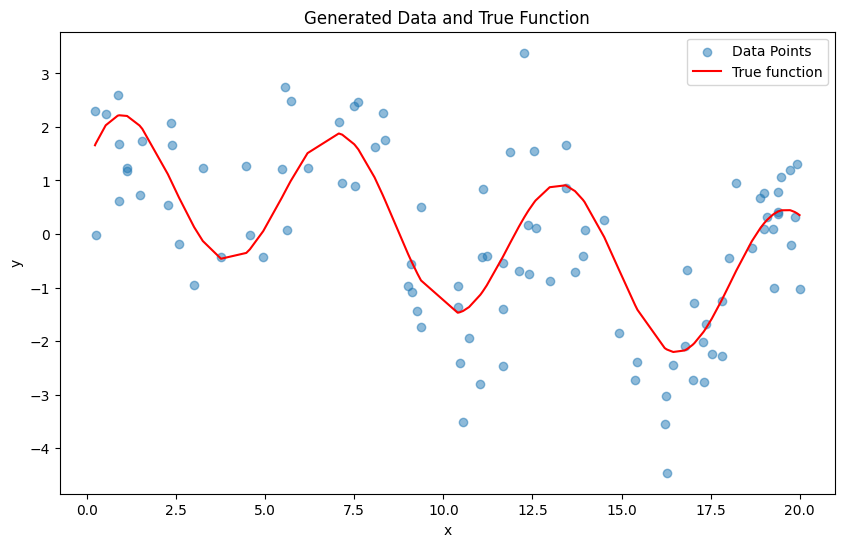
\includegraphics[width=\textwidth]{figures/data.png} 
        \caption{Non-linear data generation}
        \label{data}
    \end{minipage}\hfill
    \begin{minipage}{0.55\textwidth}
        \centering
        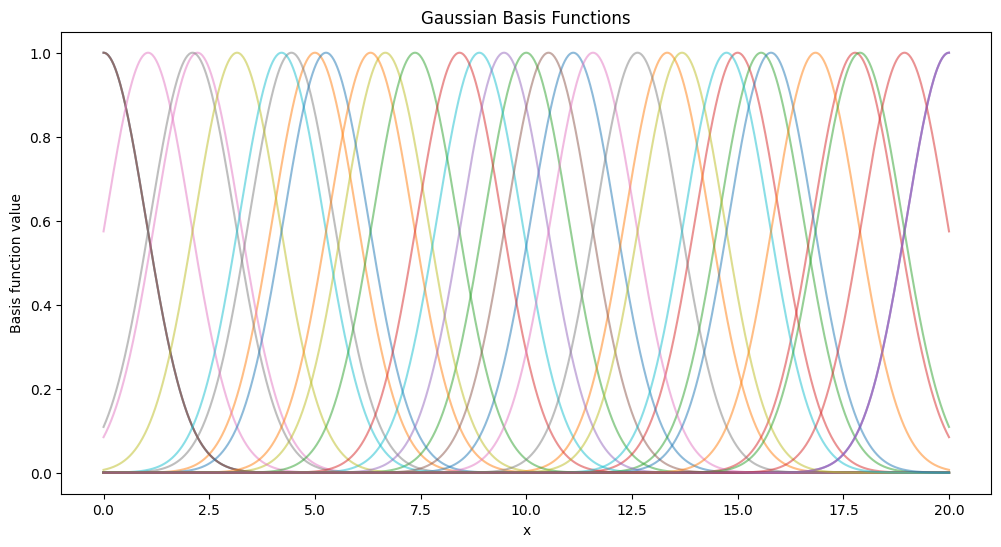
\includegraphics[width=\textwidth]{figures/gaussian_basis.png} 
        \caption{Gaussian basis for range of generated data}
        \label{gaussian}
    \end{minipage}
\end{figure}
Where $x$ is uniformly sampled from the range $[0, 20]$, and $\epsilon$ is Gaussian noise with mean 0 and variance 1. See Figure \ref{data}, the scatter plot of the generated data shows the noisy observations along with the true underlying function. The noise in the data simulates real-world measurement errors, adding complexity to the approximation task.
\begin{figure}[H]
    \centering
    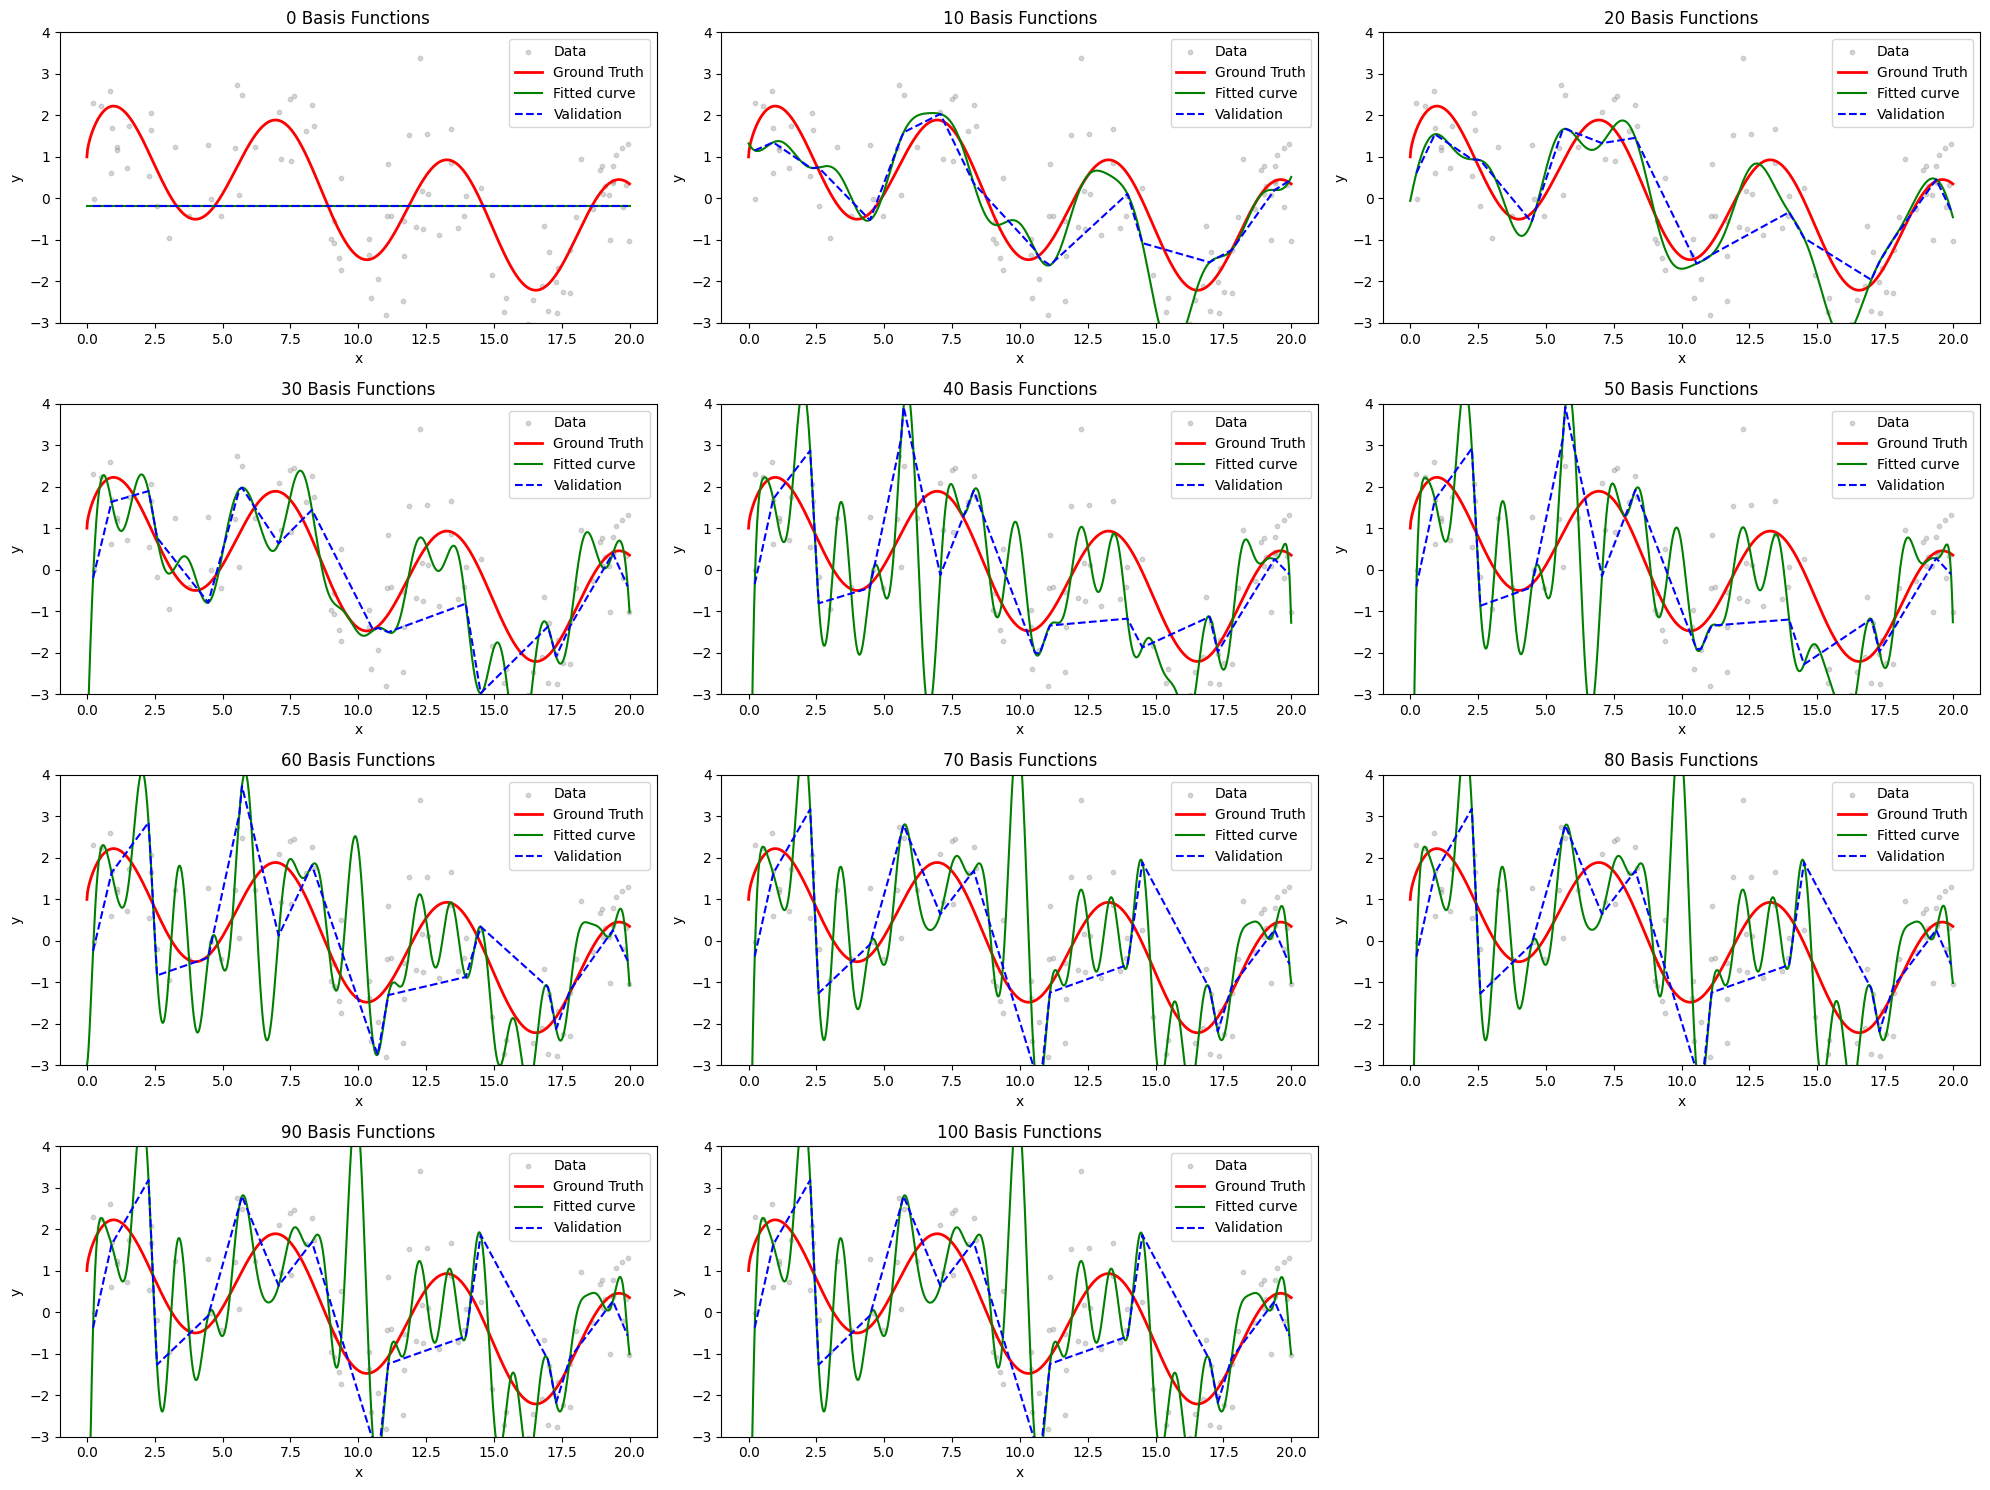
\includegraphics[width=0.95\linewidth,height=0.3\textheight]{figures/gaussian_data.png} 
    \caption{LinearRegression model fitting with Gaussian function at the range for 0,10,20, ..., 100}
    \label{gaussian data}
\end{figure}

\paragraph{Gaussian Basis Functions}
To explore the Gaussian basis function, we transform the original input features by using Gaussian basis functions of the form:
\[
\varphi(x, \mu, \sigma) = \exp\left(-\frac{(x - \mu)^2}{2\sigma^2}\right)
\]
Where $\mu$ is the mean of the Gaussian and $\sigma$ is the standard deviation. We fix $\sigma = 1$ and vary the number of basis functions from 0 to 100, with their centers ($\mu$) evenly spaced across the input range. Shown in Figure \ref{gaussian}, demonstrates how these functions can capture local patterns in the data. Each basis function responds to inputs near its center and to distant inputs.

\paragraph{Model Fitting}
We split the data to train and validation sets and implemented a linear regression class that fits the model using the pseudoinverse method with train data. Here, we can visualize the fitted curves with training sets and validation sets alongside the true function and the noisy data points after fitting multiple models, shown in Figure \ref{gaussian data}, each with a different number of basis functions (0, 10, 20, ..., 100).

\begin{figure}[H]
    \centering
    \begin{minipage}{0.45\textwidth}
        \centering
        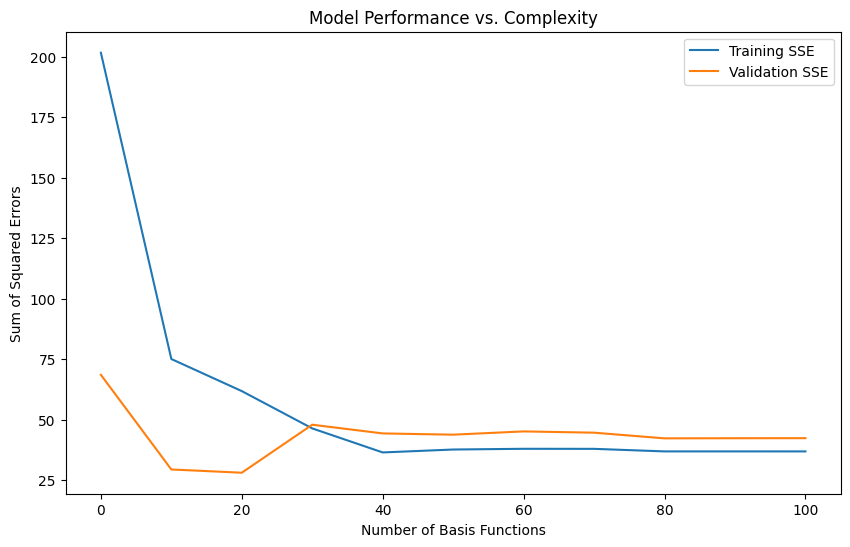
\includegraphics[width=\linewidth]{figures/complexity.png} 
        \caption{SSE for fitted models in range of Gaussian basis}
        \label{SSE}
    \end{minipage}
    \centering
    \begin{minipage}{0.50\textwidth}
        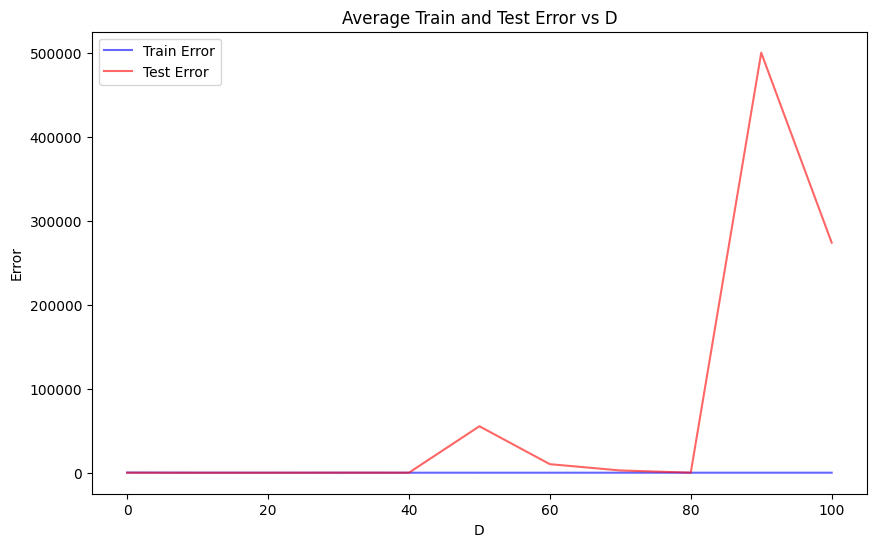
\includegraphics[width=\linewidth]{figures/average_error.png} 
        \caption{Bias-Variance Trade-off}
        \label{error_compare}
\end{minipage}

\end{figure}
\paragraph{Model Selection}
To select optimal model complexity, we again split the data into training and validation sets. Then we compute the Sum of Squared Errors (SSE) for each model on both sets. See Figure \ref{SSE} and Table \ref{SSE_table}, the results show a clear pattern of model performance across different numbers of Gaussian basis functions. With 0 basis functions, both training and validation SSE are high. As the number of basis functions increases, we observe a rapid decrease in both training and validation SSE. The optimal model complexity is achieved with 20 basis functions, where the validation SSE reaches its minimum of 28.14.


\subsection{Conclusion and Discussion}
By plotting SSE on both sets, we observed that 20 Gaussian basis functions provide the optimal balance between fitting the data and generalizing to unseen points. Models with fewer basis functions (0-10) showed clear underfitting, with high SSE values for both training and validation sets. Conversely, models with more than 20 basis functions exhibited overfitting, with decreasing training SSE but increasing validation SSE. Also, it is worth mentioning that model performance stabilized for very high numbers of basis functions (80-100), suggesting inherent regularization in our approach. Interestingly, this task demonstrates that very complex models may not perform much worse than moderately complex ones in some cases, possibly due to implicit regularization in the fitting procedure. It is important to note that input transformations can enable simple models to capture complex relationships (Myung et al., 2000)\ref{model_complexity}, and they can provide a clear illustration of the bias-variance trades-off.


\section{Task 2: Bias-Variance Tradeoff with Multiple Fits}

\subsection{Introduction}
In Task 2, we aim to understand the balance between a model's ability to capture bias and variance, which is crucial for building effective predictive models. This task explores the bias-variance trade-off in the context of non-linear function approximation using Gaussian basis functions.

\subsection{Methodology}
we extend our exploration of Gaussian basis function regression by repeating the process 10 times with resampled data. For each iteration, we generate 100 new data points from the same non-linear function as Task 1 data generation. We then fit linear regression models using Gaussian basis functions with different ranges as well.

\begin{figure}[H]
    \centering
    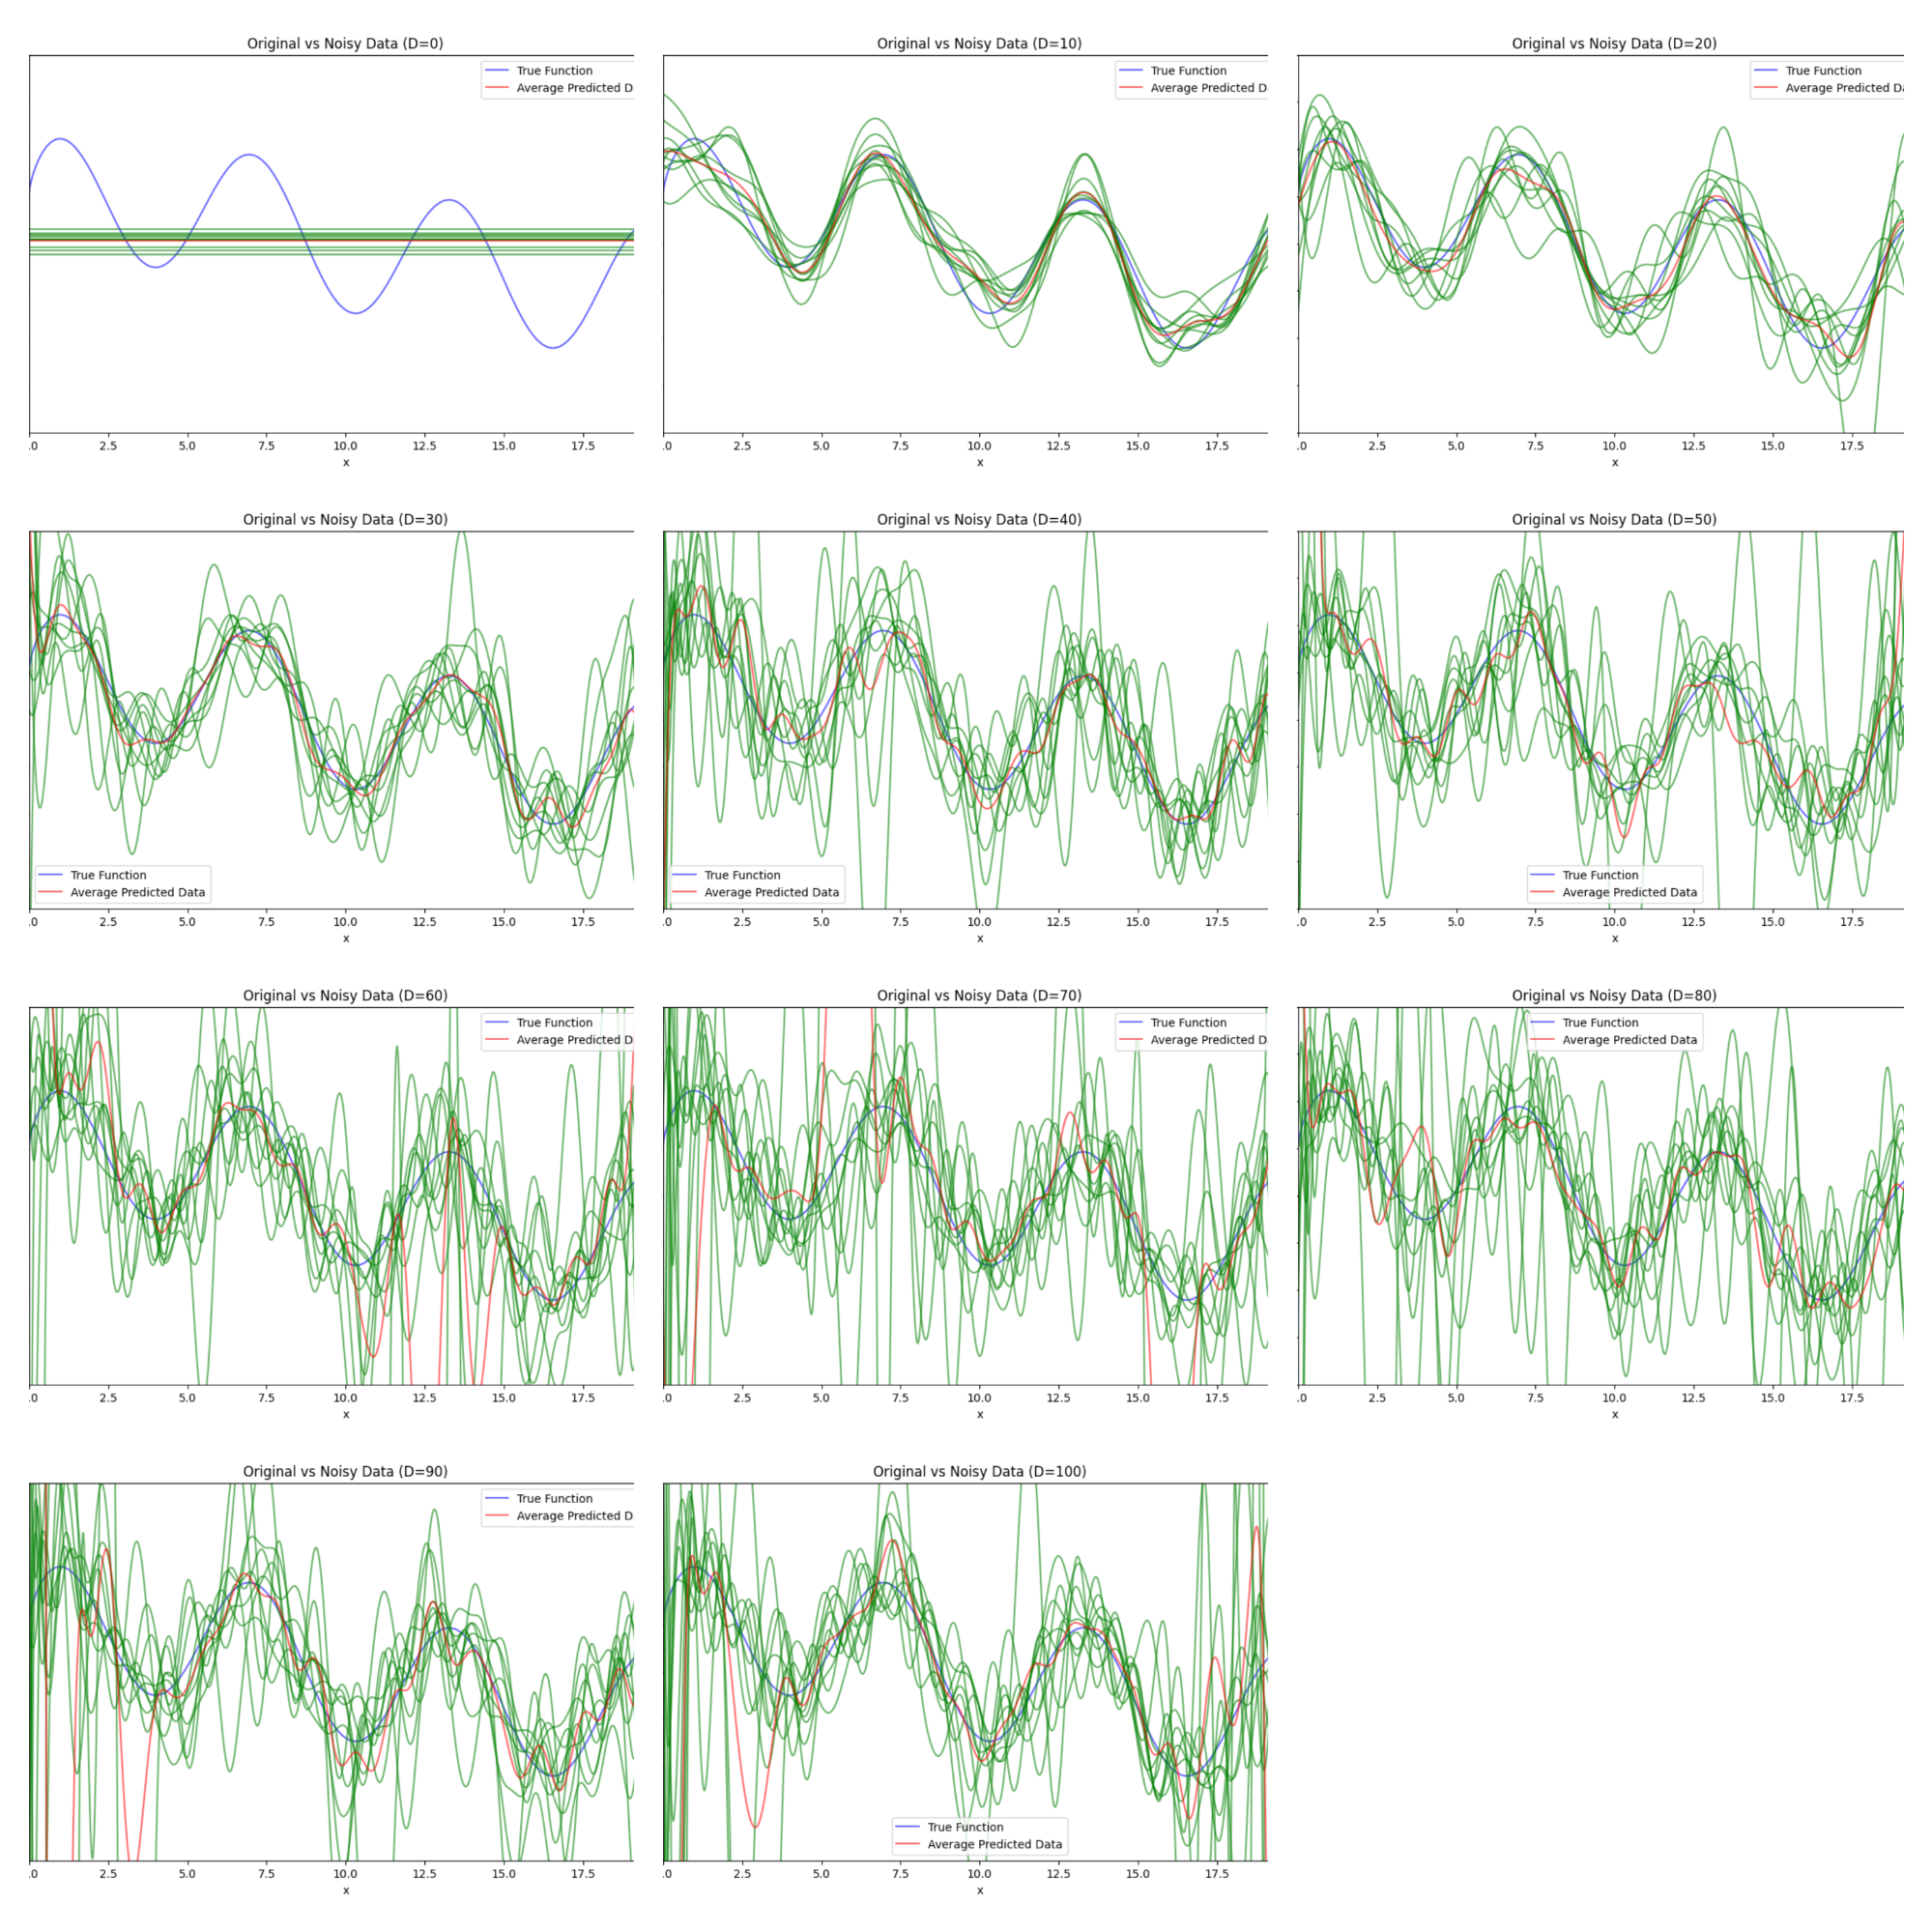
\includegraphics[width=0.9\linewidth,height=0.4\textheight]{figures/bias_variance.jpg} 
    \caption{Bias-Variance Trade-off}
    \label{bias_variance}
\end{figure}

As Figure \ref{bias_variance} illustrated, the true underlying function (blue line), and the average of the 11 fitted models (red line) on the same graph. This visualization is created for each level of model complexity. Additionally, we compute and plot the average training and test errors across the 11 iterations for each level of complexity. Also, the model result of the average error is shown in Figure \ref{error_compare}, the plots provide a clear visualization of the bias-variance trade-off as the model complexity increases. 

\subsection{Conclusion}
The combined analysis of the error plots and the bias-variance trade-off visualizations provides a comprehensive understanding of model behavior across different levels of complexity. For low numbers of basis functions (D=0-10), we observe high bias and low variance, with the model failing to capture the underlying pattern of the data. As the number of bases increases to the range of 20-40, we see an optimal balance where the model captures the true function well. However, the error plot reveals that beyond 60, there's a dramatic increase in test error in validation sets, this is also visually confirmed in Figure \ref{bias_variance}, indicating severe overfitting. This task demonstrates that while increasing model complexity can reduce bias, it has the potential to increase variance to the point of severe overfitting. The optimal model should strike a balance, typically achieved with a moderate number of basis functions, which is around 30 in our case.

\section{Task 3: Regularization with Cross-Validation}

\subsection{Introduction}
\noindent Introduction
In this task, we implemented both \textbf{L1 (Lasso)} and \textbf{L2 (Ridge)} regularization into a linear regression model using synthetic data transformed by Gaussian basis functions. We conducted cross-validation to evaluate model performance under different values of the regularization parameter $\lambda$, ranging from $10^{-4}$ to $10^2$. Furthermore, we performed a \textbf{bias-variance decomposition} to analyze the effects of regularization on model complexity. This journal discusses each aspect of the implementation, followed by an analysis of the resulting error and bias-variance graphs.


\subsection{Methodology}
\paragraph{Implementation of L1 and L2 Regularization}
For L1 regularization (Lasso), the goal is to minimize the sum of squared residuals while also penalizing the absolute values of the weights $w$. The loss function for \textbf{L1 regularization} is given by: $J(w) = \frac{1}{2m} \sum_{i=1}^{m} \left( y^{(i)} - w^T x^{(i)} \right)^2 + \lambda \sum_{j=1}^{n} \left| w_j \right|$
Here, the first term represents the mean squared error (MSE), and the second term is the L1 penalty on the weights. The parameter $\lambda$ controls the strength of the regularization: a larger $\lambda$ forces more weights to become zero, making the model sparser.

For \textbf{L2 regularization (Ridge)}, the penalty is applied to the squared values of the weights, resulting in the following loss function: $J(w)=\frac{1}{2 m} \sum_{i=1}^m\left(y^{(i)}-w^T x^{(i)}\right)^2+\frac{\lambda}{2} \sum_{j=1}^n w_j^2$

In this case, the second term is the L2 penalty, which tends to shrink the weights towards zero without making them exactly zero. Again, $\lambda$ controls the regularization strength, helping reduce over-fitting by penalizing large weights.

Both these regularization methods were implemented by modifying the loss functions accordingly and using gradient descent to update the weights iterative.

\paragraph{Cross-Validation for Model Assessment}
For each $\lambda$ value, we used \textbf{10-fold cross-validation} to calculate the training and validation \textbf{MSE}. The MSE for the training and validation sets is computed as: $\mathrm{MSE}=\frac{1}{m} \sum_{i=1}^m\left(y^{(i)}-\hat{y}^{(i)}\right)^2$
where $y^{(i)}$ represents the true value and $\hat{y}^{(i)}$ is the predicted value. By averaging the MSE across all folds, we obtained a reliable estimate of the model's generalization performance.

\paragraph{Bias-Variance Decomposition}
To analyze the bias-variance trade-off, we decomposed the total error into three components: bias, variance, and noise variance. The bias squared is calculated as: $\operatorname{Bias}^2=\frac{1}{m} \sum_{i=1}^m\left(\mathbb{E}\left[\hat{y}^{(i)}\right]-y^{(i)}\right)^2$


Here, $\mathbb{E}\left[\hat{y}^{(i)}\right]$ is the expected prediction over multiple datasets, and $y^{(i)}$ is the true output.

The variance measures the variability of the model's predictions across different datasets:
$\text { Variance }=\frac{1}{m} \sum_{i=1}^m \mathbb{E}\left[\left(\hat{y}^{(i)}-\mathbb{E}\left[\hat{y}^{(i)}\right]\right)^2\right]
$
Finally, the total error combines the bias, variance, and noise variance: $\text { Total Error }=\text { Bias }^2+\text { Variance }+\sigma_{\text {noise }}^2$

where $\sigma_{\text {noise }}^2$ represents the inherent noise in the data.

\begin{itemize}
    \item \textbf{L2 regularization} \\
    As $\lambda$ increased, the bias increased, and the variance decreased. This is expected because larger $\lambda$ values restrict model flexibility, leading to simpler models with higher bias and lower variance. The total error increased as the model became overly simplistic at high $\lambda$ values.

    \item \textbf{L1 regularization} \\
     As $\lambda$ increased, the bias also increased while variance decreased. However, the variance remained more stable compared to L2 regularization, suggesting that L1 regularization helped retain some model flexibility even at larger $\lambda$ values.
\end{itemize}

\paragraph{Selection of Optimal $\lambda$}
Based on the validation error plots, the optimal $\lambda$ for both regularization methods was selected where the validation error was minimized. For L2 regularization, the optimal $\lambda$ value lay in the middle of the range (around $\lambda \approx 10$ ), where the model achieved a balance between under-fitting and over-fitting. Similarly, for L1 regularization, the optimal $\lambda$ value was also around $\lambda \approx 10$, where the validation error curve flattened.

The bias-variance decomposition further supported these choices. At the optimal $\lambda$ values, both the bias and variance were balanced, and the total error was minimized.

\subsection{Conclusion}
\begin{figure}[h]
    \centering
    \begin{minipage}{0.50\textwidth}
        \centering
        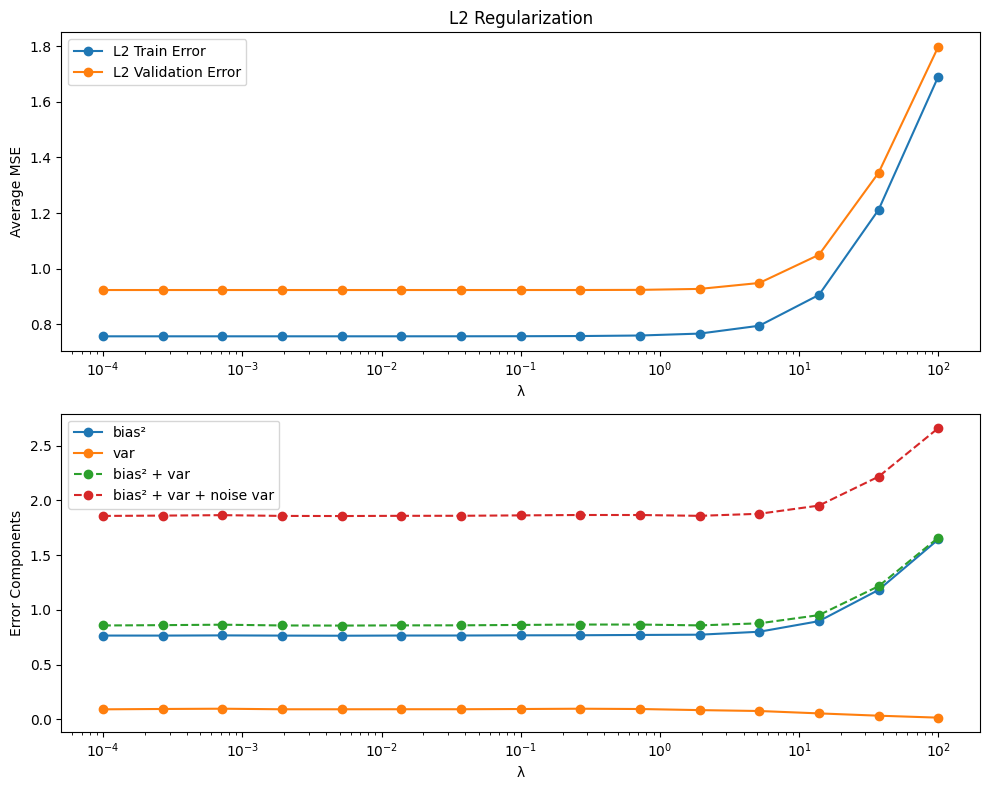
\includegraphics[width=\textwidth]{figures/L2_Regularization.png} 
        \caption{L2 Regularization}
        \label{L2}
    \end{minipage}\hfill
    \begin{minipage}{0.50\textwidth}
        \centering
        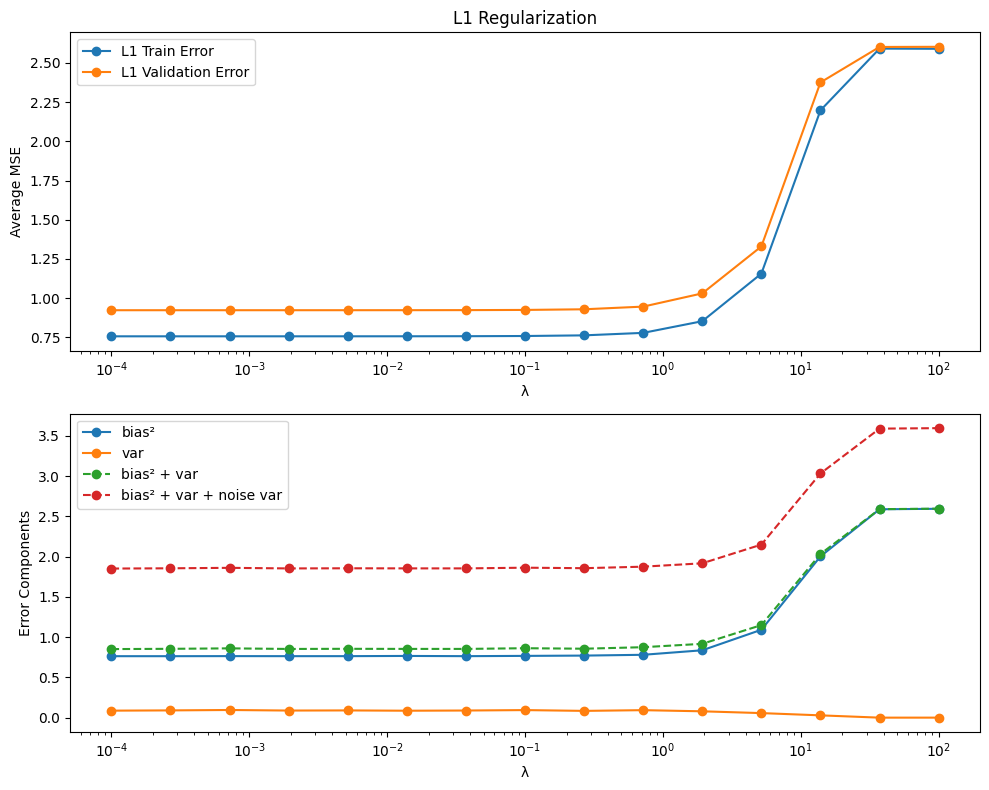
\includegraphics[width=\textwidth]{figures/L1_Regularization.png} 
        \caption{L1 Regularization}
        \label{L1}
    \end{minipage}
\end{figure}

By plotting the training and validation errors as a function of $\lambda$, we observed that:\\
$\bullet$ For small $\lambda$, both L1 and L2 regularization resulted in low training errors but higher validation errors, indicating over-fitting.\\
$\bullet$ As $\lambda$ increased, the training error rose, and the validation error initially decreased before rising again at very large $\lambda$, indicating under-fitting.
\\
The bias-variance decomposition further confirmed this, showing that:\\
$\bullet$ For small $\lambda$, variance was high, while bias was low, leading to over-fitting.\\
$\bullet$ As $\lambda$ increased, the bias increased while the variance decreased, balancing the two components and minimizing the total error at an intermediate value of $\lambda$.

The optimal $\lambda$ was chosen where the validation error and total error were minimized, balancing both bias and variance effectively.

In conclusion, the implementation of L1 and L2 regularization successfully controlled the complexity of the model, helping reduce over-fitting for small $\lambda$ values and under-fitting for large $\lambda$ values. Cross-validation provided a reliable way to assess the model's performance and choose the optimal $\lambda$ for both regularization types. The\textbf{ train-validation error plots} 
and \textbf{bias-variance decomposition} illustrated the impact of regularization on model performance.


\section{Task 4: Effect of L1 and L2 Regularization on Loss}

\subsection{Introduction}
\noindent This task examines the effects of L1 (Lasso) and L2 (Ridge) regularization on linear regression models using synthetic data. We investigate regularization strengths ($\lambda$) ranging from 0.01 to 10. The analysis involves visualizing loss function contours and gradient descent paths for each regularization type and strength. This approach allows for a comparative assessment of how L1 and L2 regularization influences the optimization landscape and convergence behavior in linear regression problems. The findings provide insights into the characteristics and impacts of these regularization techniques on model fitting and parameter estimation.

\subsection{Methodology}
\paragraph{Data Generation}
We generate a synthetic dataset of 50 samples using the model y = −4x + 10 + 2$\epsilon$, where x is uniformly distributed between 0 and 10, and $\epsilon$ is Gaussian noise with mean 0 and variance 1.

\paragraph{Regularization Implementation}
We implement both L1 and L2 regularization methods, defining loss functions as combinations of Mean Squared Error (MSE) and the respective regularization terms. A GradientDescent class performs the optimization, running until convergence or a maximum number of iterations is reached, while recording the optimization history for visualization purposes.

\paragraph{Experimental Design and Visualization}
We compare L1 and L2 regularization using four regularization strengths ($\lambda$): 0.01, 0.1, 1, and 10. For each combination, we visualize the optimization landscape through loss function contours and overlay gradient descent paths to illustrate the optimization trajectory.

\subsection{Conclusion}
\begin{figure}[h]
    \centering
    \begin{minipage}{1\textwidth}
        \centering
        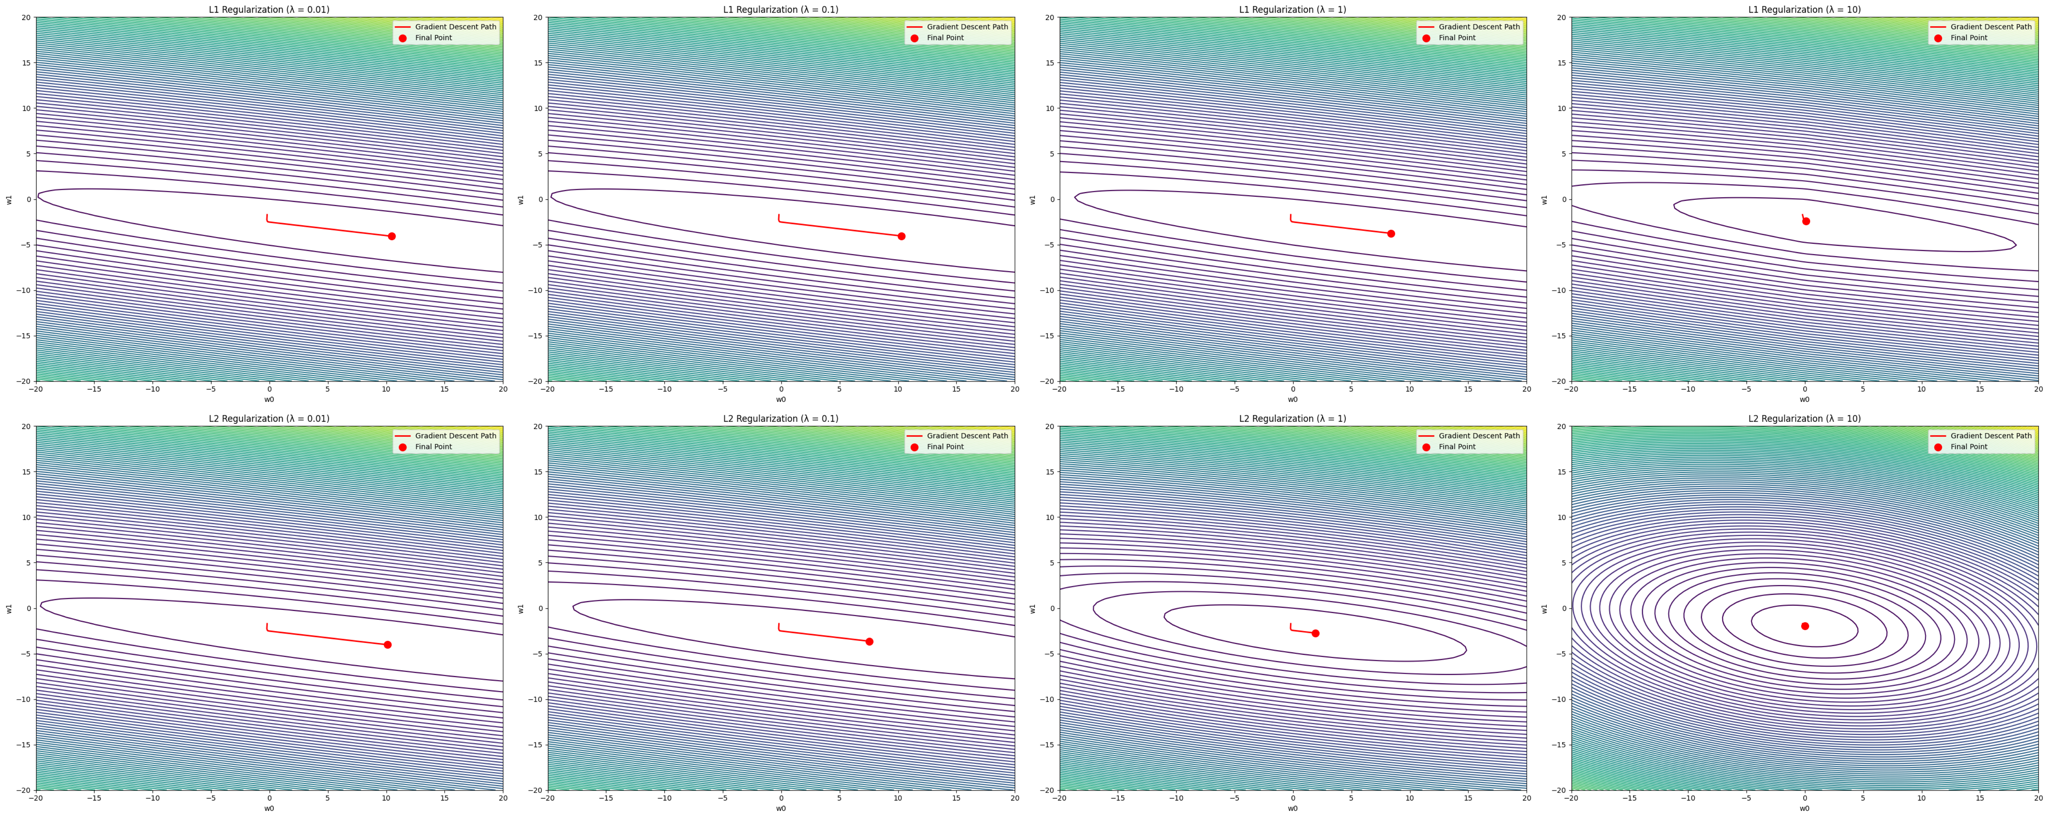
\includegraphics[width=\textwidth]{figures/T4.png} 
        \caption{L1 and L2 Regularization ($\lambda$ = 0.01, 0.1, 1, 10)}
    \end{minipage}
\end{figure}

By plotting the loss function contours and gradient descent paths, we observed the following:

\paragraph{L1 Regularization and Sparsity}
L1 regularization encourages sparsity by driving some weights to exactly zero. This is evident in the plots, especially for higher $\lambda$ values (1 and 10), where the optimization paths move towards the axes. The final points for $\lambda = 10$ in L1 regularization are very close to one axis, indicating that one weight is nearly zero. The diamond-shaped contours of the loss landscape, particularly pronounced at higher $\lambda$ values, further illustrate this sparsity-inducing property.

\paragraph{L2 Regularization and Weight Penalization}
L2 regularization typically penalizes large weights but does not promote sparsity as strongly as L1, though this distinction is not clearly evident in these specific plots. For lower $\lambda$ values, both L1 and L2 show similar behavior. At higher $\lambda$ values, particularly $\lambda$=10, the L2 plot shows more circular contours, indicating uniform penalization in all directions. However, contrary to typical expectations, the L2 final point for $\lambda$=10 is closer to an axis than the L1 point. This unexpected result highlights that while regularization techniques have general tendencies, their effects can vary in specific instances and may require more extensive analysis to clearly demonstrate their characteristic behaviors.

\paragraph{Effect of $\lambda$ on Optimization Paths and Loss Landscapes}
As $\lambda$ increases from 0.01 to 10, both regularization types show stronger effects:

\begin{itemize}
    \item For L1:
    \begin{itemize}
        \item The paths become shorter and more curved, moving along or towards the axes.
        \item The loss landscape contours become more diamond-shaped, emphasizing the sparsity-inducing effect.
    \end{itemize}
    \item For L2:
    \begin{itemize}
        \item The paths also shorten but remain more direct.
        \item The loss landscape contours become more circular, illustrating the uniform penalization of weights.
    \end{itemize}
\end{itemize}

In both cases, higher $\lambda$ values lead to quicker convergence, indicated by shorter optimization paths. However, L1 paths tend to move along axes at higher $\lambda$ values, while L2 paths don't show this axis-aligned preference.

\section{Discussion and Conclusion}



\section{Statement of Contributions}

All members contributed equally to this project. We each completed the lab independently and then combined our individual work and code to produce the final report.

\newpage
\bibliographystyle{unsrt}  
%\bibliography{references}  %%% Remove comment to use the external .bib file (using bibtex).
%%% and comment out the ``thebibliography'' section.

%%% Comment out this section when you \bibliography{references} is enabled.
\begin{thebibliography}{1}

\bibitem{model complexity} Myung, I. J. (2000). The importance of complexity in model selection. Journal of mathematical psychology, 44(1), 190-204.
\label{model_complexity}

\bibitem{Lecture notes} Prémont-Schwarz, I. (2023). Gradient Descent. COMP 551, McGill University.\label{ref:lectures}


\end{thebibliography}

\begin{appendices}

\section{Default Model Parameters} \label{app:default-parameters}

\begin{table}[H]
    \centering
    \vspace{7pt} % Adjust the value as needed to control the amount of space
    \renewcommand{\arraystretch}{1.5}
    \begin{tabular}{|c|c|c|c|c|c|}
        \hline
        Model  & Max iteration & Batch Size & Learning Rate & Epsilon & Regularization Term \\
        \hline
        Linear Regression with SGD & 1500 & 16 & 1e-2 & 1e-5 & 0 \\
        Logistic Regression & 2000 & 16 & 1e-3 & 1e-7 & 0.1 \\
        \hline
    \end{tabular}
\end{table}

\section{Experiment 3}

\subsection{Training Loss History of Linear Regression with data size} \label{app:loss-history-sgd}

\begin{table}[h]
    \centering
    \begin{minipage}{0.45\textwidth}  % Adjust the width as needed
        \centering
        \begin{tabular}{|c|c|}
            \hline
            \textbf{Training Size (Proportion)} & \textbf{MSE Loss} \\
            \hline
            0.2  & 233.8436 \\
            0.3  & 100.6199 \\
            0.4  & 162.3182 \\
            0.5  & 11.3937  \\
            0.6  & 7.1098   \\
            0.7  & 0.0650   \\
            0.8  & 0.0635   \\
            \hline
        \end{tabular}
        \vspace{7pt}
        \caption{Linear in Different Training Set Sizes}
        \label{linear train size}
    \end{minipage}
    \hfill
    \begin{minipage}{0.45\textwidth}  % Adjust the width as needed
        \centering
        \begin{tabular}{|c|c|}
            \hline
            \textbf{Training Size (Proportion)} & \textbf{MSE Loss} \\
            \hline
            0.2  & 0.3201 \\
            0.3  & 0.3198 \\
            0.4  & 0.3195 \\
            0.5  & 0.3213  \\
            0.6  & 0.3191   \\
            0.7  & 0.3189   \\
            0.8  & 0.3198   \\
            \hline
        \end{tabular}
        \vspace{7pt}
        \caption{Logistic in Different Training Set Sizes}
        \label{logistic train size}
    \end{minipage}
\end{table}

\subsection{Final Loss, Mean Loss and Min Loss in Linear Regression model with different mini-batch SGD} \label{app:loss-history-sgd-log}
\begin{minipage}{0.45\textwidth}  % Adjust width as needed
        \centering
        \begin{tabular}{|c|c|c|}
            \hline
            {Number of Bases} & {Training SSE} & {Validation SSE} \\
            \hline
             0  & 201.64  & 68.58  \\
            10  &  75.11  & 29.48  \\
            20  &  61.85  & 28.14  \\
            30  &  46.44  & 47.97  \\
            40  &  36.52  & 44.37  \\
            50  &  37.72  & 43.86  \\
            60  &  38.02  & 45.20  \\
            70  &  38.00  & 44.68  \\
            80  &  36.94  & 42.33  \\
            90  &  36.95  & 42.39  \\
           100  &  36.94  & 42.41  \\
            \hline
        \end{tabular}\\
        \vspace{0.3cm}
        \textbf{Optimal number of basis functions: 20}
        \captionof{table}{Training and validation SSE }
        \label{SSE_table}
    \end{minipage}


\end{appendices}

\end{document}

